\documentclass[11pt,letterpaper]{article}
\usepackage[utf8]{inputenc}
\usepackage[spanish]{babel}
\usepackage[margin=1in]{geometry}
\usepackage{amsmath,amssymb}
\newcommand*{\QEDB}{\hfill\ensuremath{\square}}%
\newcommand\tab[1][1cm]{\hspace*{#1}}
\DeclareMathOperator{\Exists}{\exists}
\DeclareMathOperator{\Forall}{\forall}
\title{Tarea 2 Programación Declarativa}
\usepackage{listings}
\usepackage{color}
\definecolor{codegreen}{rgb}{0,0.6,0}
\definecolor{codegray}{rgb}{0.5,0.5,0.5}
\definecolor{codepurple}{rgb}{0.58,0,0.82}
\definecolor{backcolour}{rgb}{0.95,0.95,0.92}

\lstdefinestyle{mystyle}{
    backgroundcolor=\color{backcolour},   
    commentstyle=\color{codegreen},
    keywordstyle=\color{magenta},
    numberstyle=\tiny\color{codegray},
    stringstyle=\color{codepurple},
    basicstyle=\footnotesize,
    breakatwhitespace=false,         
    breaklines=true,                 
    captionpos=b,                    
    keepspaces=true,                 
    numbers=left,                    
    numbersep=5pt,                  
    showspaces=false,                
    showstringspaces=false,
    showtabs=false,                  
    tabsize=2
}
\lstset{
style=mystyle,
literate={á}{{\'a}}1
        {ã}{{\~a}}1
        {é}{{\'e}}1
        {ó}{{\'o}}1
        {í}{{\'i}}1
        {ñ}{{\~n}}1
        {¡}{{!`}}1
        {¿}{{?`}}1
        {ú}{{\'u}}1
        {Í}{{\'I}}1
        {Ó}{{\'O}}1
}

\usepackage{graphicx}
\usepackage{enumerate}
\usepackage{enumitem}

\usepackage{longtable}
\usepackage{hyperref}
\usepackage{commath}
\begin{document}
\title{\vspace{-1.5cm}
	Tarea 2\\
    \large Universidad Nacional Autónoma de México\\
    Facutlad de Ciencias\\
    Programación Declarativa\\
}
\author{
	Fong Baeza Luis Fernando Yang\\
    \texttt{fernandofong@ciencias.unam.mx}
    \and 
    Ávila Valdovinos Sebastián\\
    \texttt{sevbald@ciencias.unam.mx}
    }
\date{26 de Marzo 2018}
\maketitle
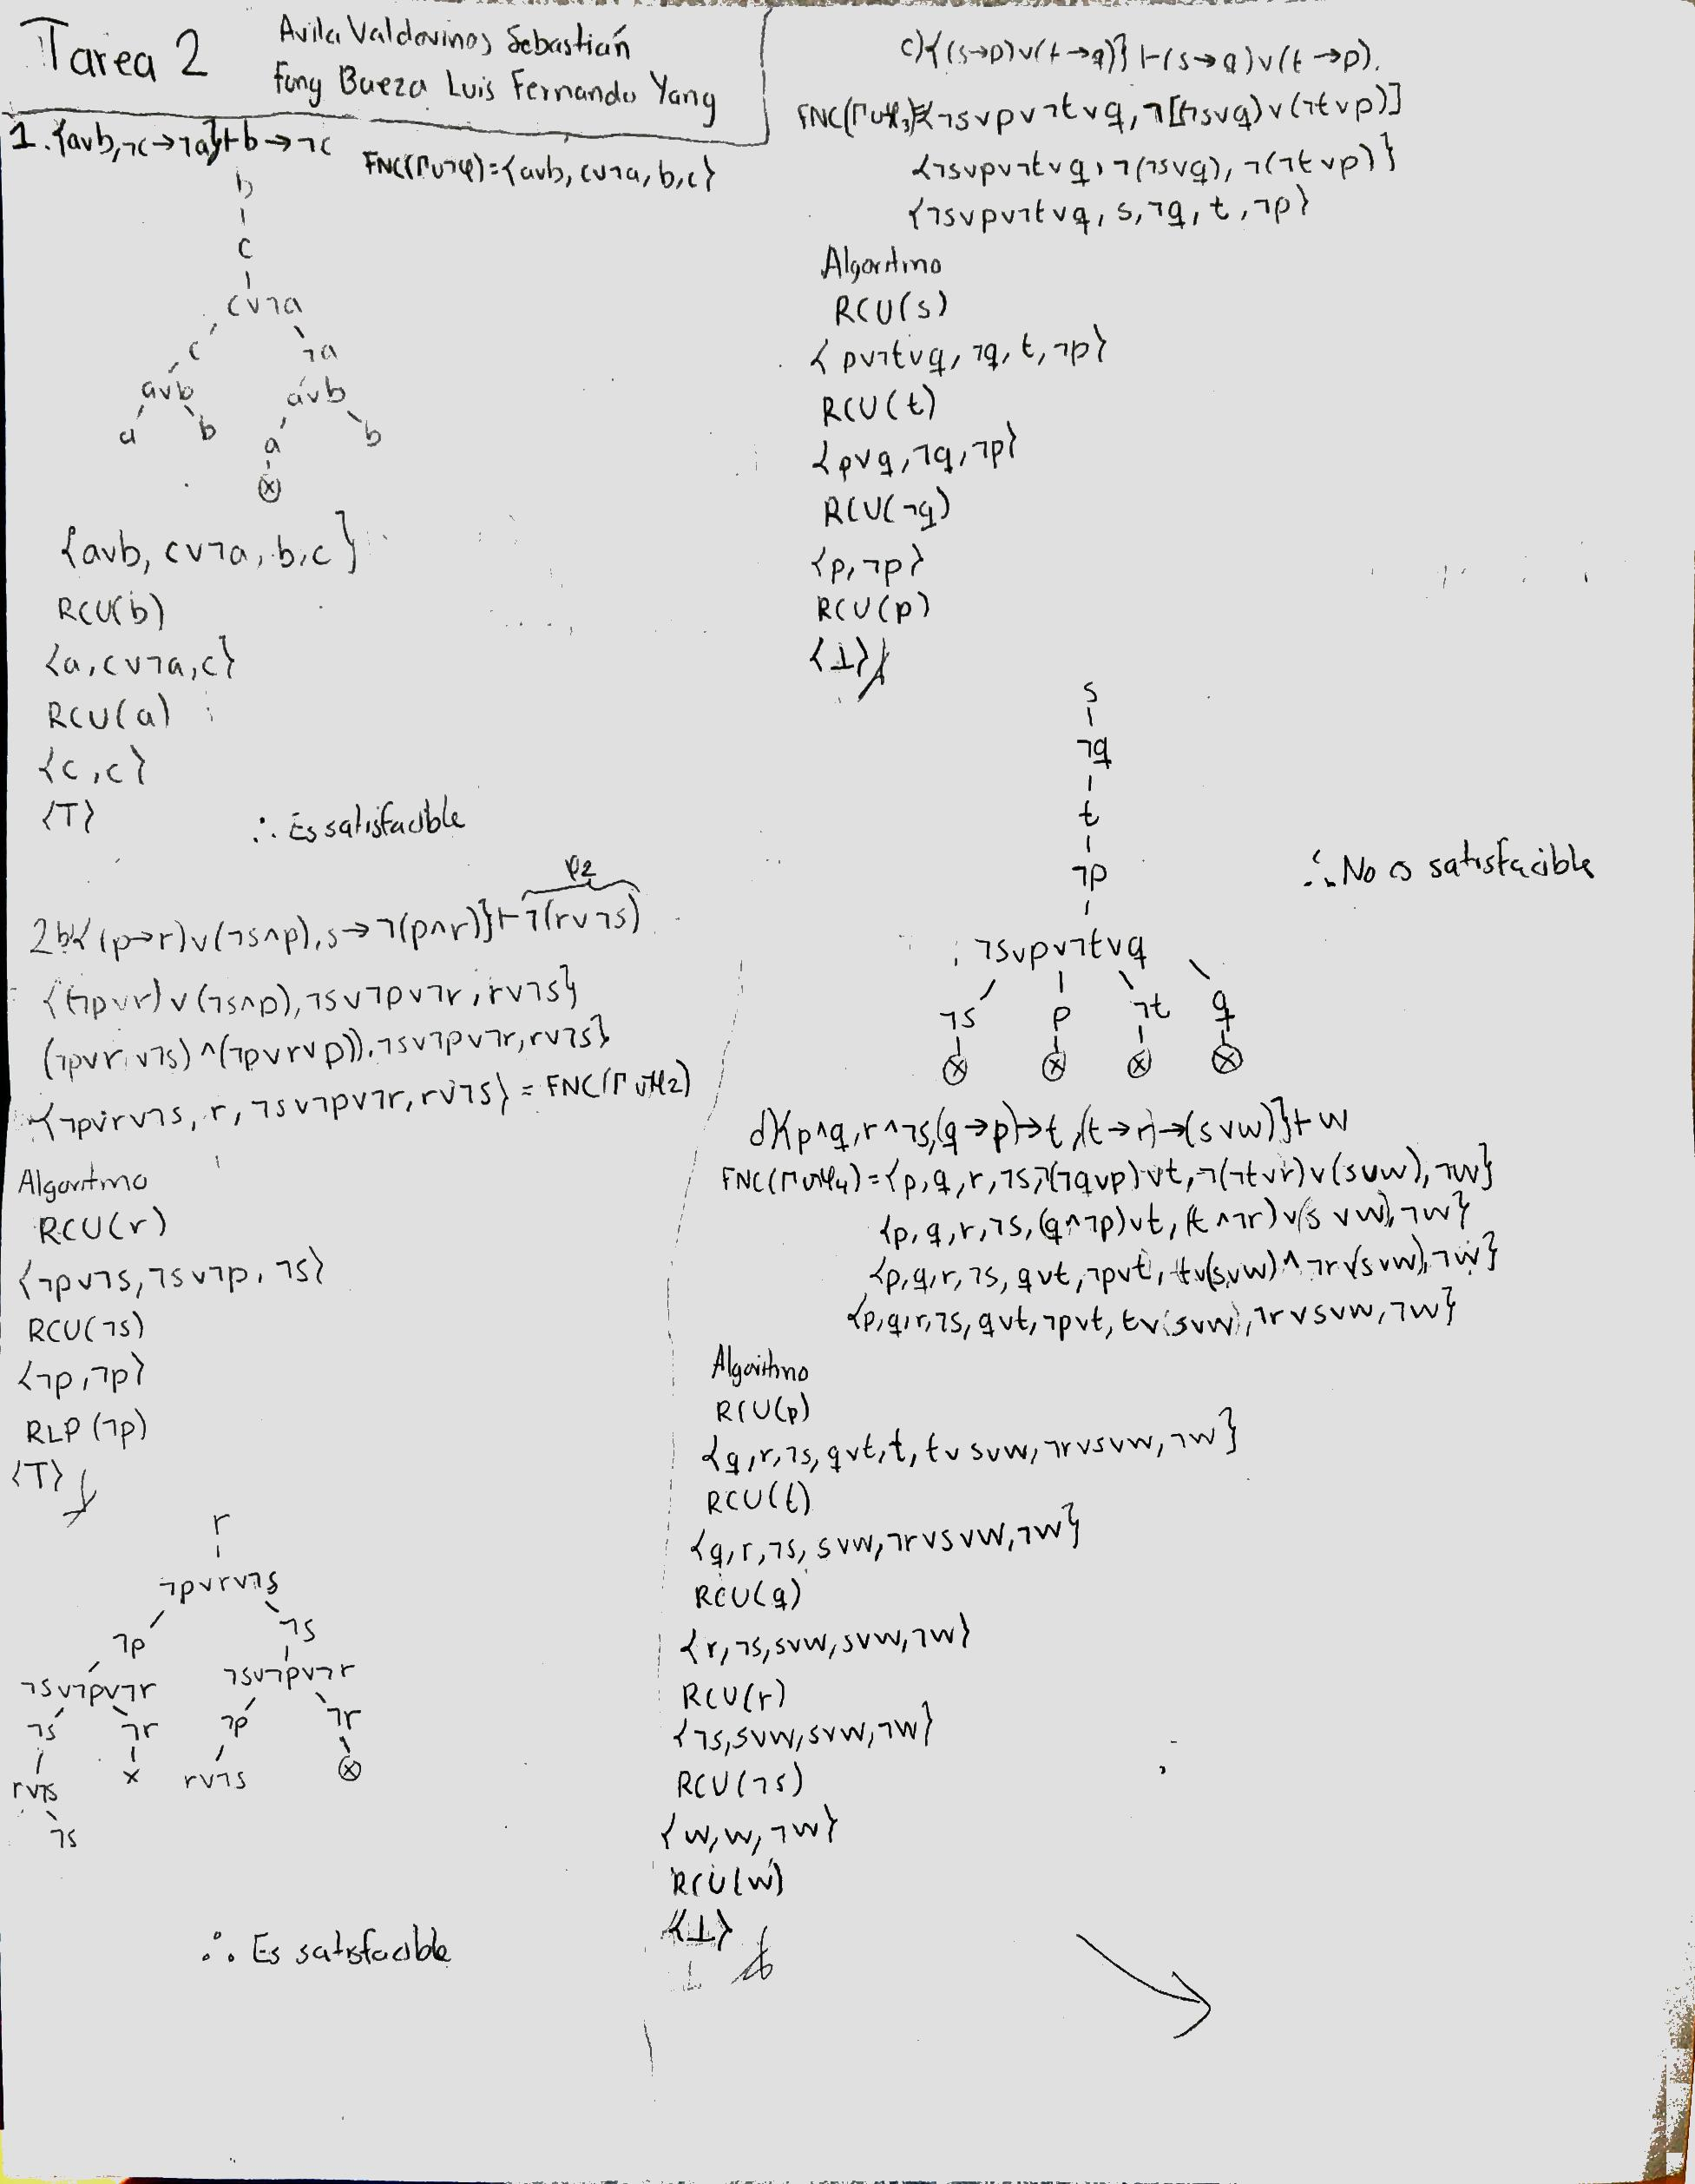
\includegraphics[width=0.8\textwidth]{parte1.jpg}\\
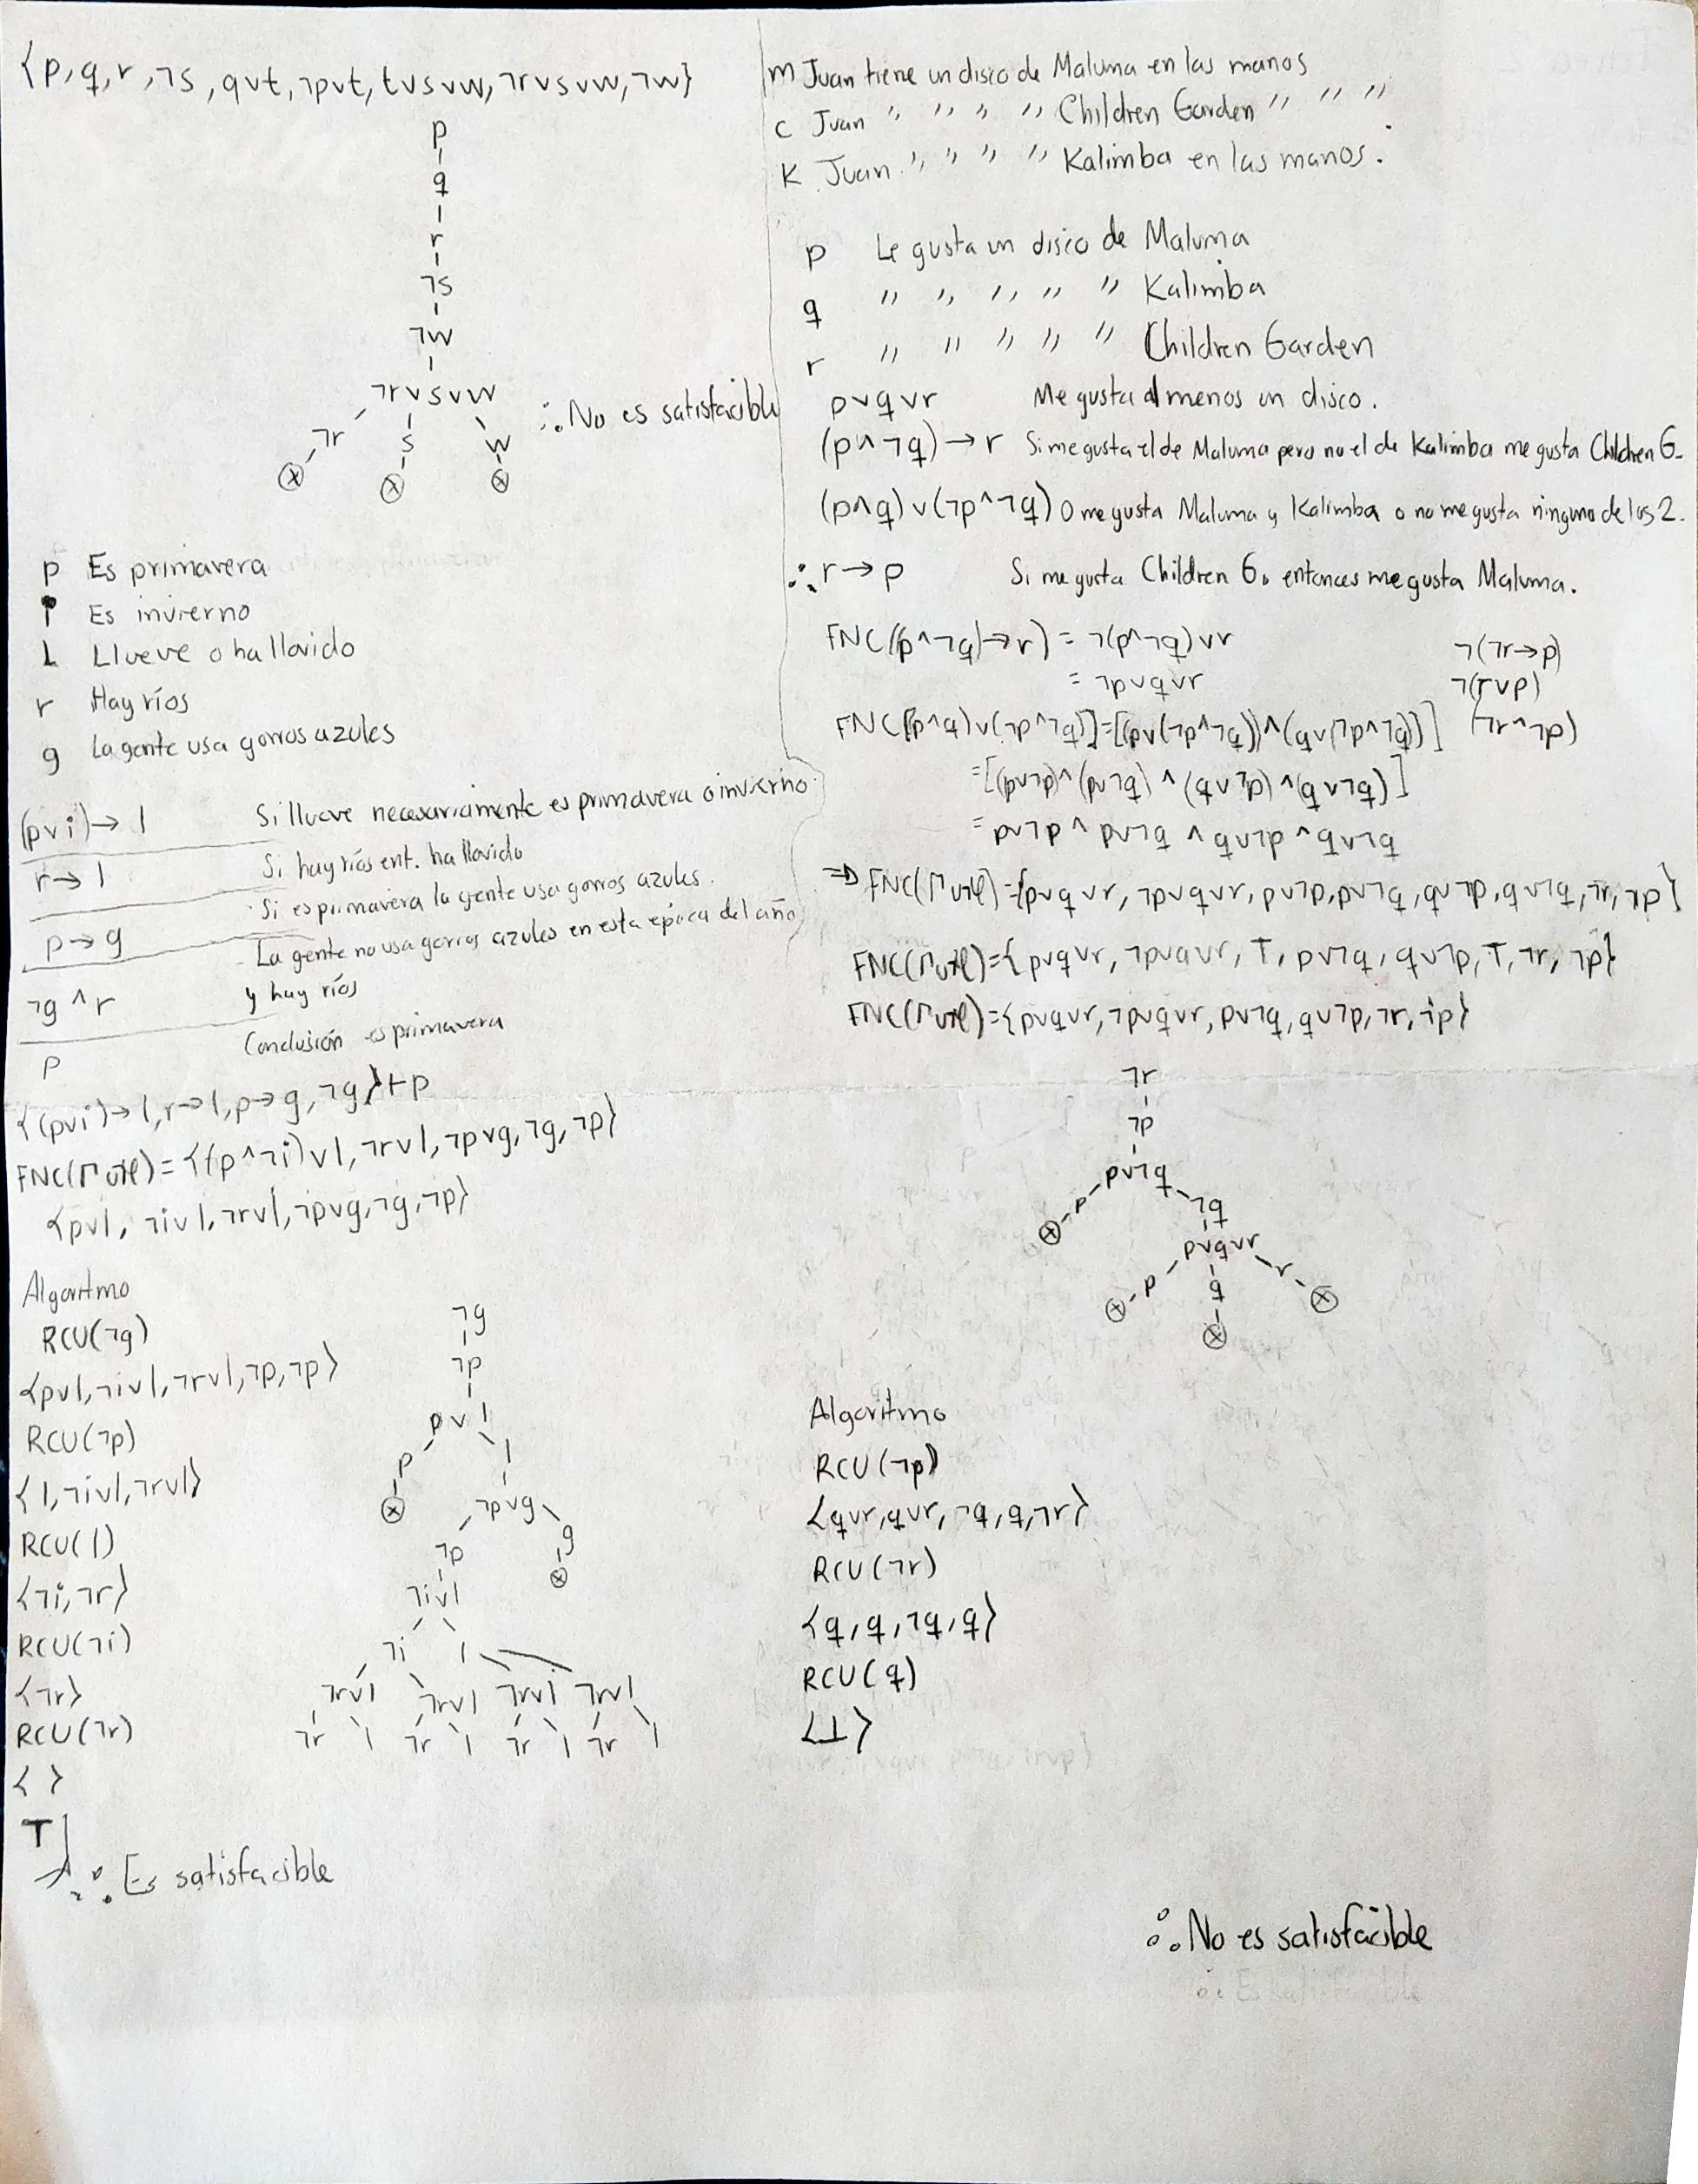
\includegraphics[width=0.9\textwidth]{parte2.jpg}
\end{document}
